\section{Tools und Arbeitsabläufe}

Innerhalb des Cloud-Team wird jedes IT-Projekt agil nach der Scrum-Methode entwickelt.
Scrum ist ein Framework für die Entwicklung komplexer Softwareprodukte.
Sie wird von ihren Schöpfern als "ganzheitlicher, iterativer Rahmen definiert, der sich auf gemeinsame Ziele konzentriert, indem er produktiv und kreativ Produkte von höchstmöglichem Wert liefert" \cite{ScrumGuide}.
13
Es basiert auf der Unterteilung eines Projekts in "Zeit Boxen", sogenannte Sprints, die von ein paar Stunden bis zu einem Monat dauern können (in unserem Team dauert es eine Woche)

\subsection{Scrum}

Das Cloud-Team wendet mehrere Scrum-Methoden zur Verbesserung der
Software-Entwicklung an:

\subsubsection{Sprint Meeting}
Zu Beginn jedes Sprints trifft sich das Cloud-Team, um die verschiedenen Aufgaben für den nächsten Sprint zu planen und diese in Tickets zu organisieren.
Sie finden jeden Montag um 10 Uhr morgens statt und dauern durchschnittlich 30 Minuten.

\subsubsection{Retro Meeting}
Diese Treffen finden einmal pro Woche statt und ermöglichen jedem Teamentwickler, die guten und schlechten Punkte der vergangenen Woche zum Ausdruck zu bringen.
Dies gibt Rückmeldung über die Stimmung im Team. Sie finden jeden Donnerstag um 13.00 Uhr statt und dauern durchschnittlich 45 Minuten.

\subsubsection{Kanban board}
Die Verfolgung unserer Sprint-Tickets erfolgt über eine Kanban-Tafel.
Es handelt sich dabei um ein agiles Projektmanagement-Tool, das dazu dient, die Arbeit zu visualisieren, die laufende Arbeit zu begrenzen und die Effizienz zu maximieren.
Unsere Tabelle besteht aus 6 Spalten:

\begin{itemize}
  \item \textbf{Backlog}: Tickets geplant, aber nicht bearbeitet
  \item \textbf{Open}: Tickets, die im aktuellen Sprint erledigt werden müssen
  \item \textbf{On Hold}: Geplantes, aber für unbestimmte Zeit blockiertes Ticket
  \item \textbf{In Progress}: Die Tickets, die realisiert werden
  \item \textbf{Review}: Tickets, die derzeit einer Code Review unterzogen werden
  \item \textbf{Closed}: Tickets, die validiert und im Entwicklungszweig zusammengeführt wurden
\end{itemize}

Jedes Ticket muss begleitet sein von:
\begin{itemize}
  \item \textbf{Ein Story point}: es handelt sich um eine Zahl zwischen 1 und 8, die der geschätzten Anzahl der Stunden entspricht, die für die Erstellung des Tickets benötigt werden
  \item \textbf{eine Priorität}: dem Ticket muss Vorrang eingeräumt werden (low, medium oder high)
\end{itemize}



\subsection{Tools}

Wir verwalten all diese Prozesse sowie die Verwaltung des Codes mit verschiedenen Tools:

\subsubsection{Git}

Git\footnote{\href{https://git-scm.com/}{https://git-scm.com/}} ist ein freies und quelloffenes verteiltes Versionskontrollsystem.
Es handelt sich um ein einfaches und leistungsfähiges Tool, dessen Hauptaufgabe darin besteht, die Entwicklung der Inhalte einer Baumstruktur zu verwalten.

Git ist das Tool, aber um ein kollaboratives Projekt richtig zu verwalten, braucht das Team einen Arbeitsablauf.
Das Team hat sich für Gitflow\footnote{\href{https://www.atlassian.com/git/tutorials/comparing-workflows/gitflow-workflow}{https://www.atlassian.com/git/tutorials/comparing-workflows/gitflow-workflow}} entschieden. Dieses Workflow definiert ein striktes branch-modell, das um eine Projektfreigabe herum entworfen wurde
\footnote{Stackoverflows git-flow tag Beschreibung: \href{https://stackoverflow.com/questions/tagged/git-flow}{https://stackoverflow.com/questions/tagged/git-flow}}.

Das innerhalb des Unternehmens verwendete Modell ist recht einfach. Es besteht aus einem "main"-Branch, der die für die Code-Produktion fertige Version mit den verschiedenen Versionen enthält, den "develop"-Branch, der dem Zweig entspricht, der sich auf alle "feature"-Branch bezieht:

\begin{figure}[h]
  \centering
  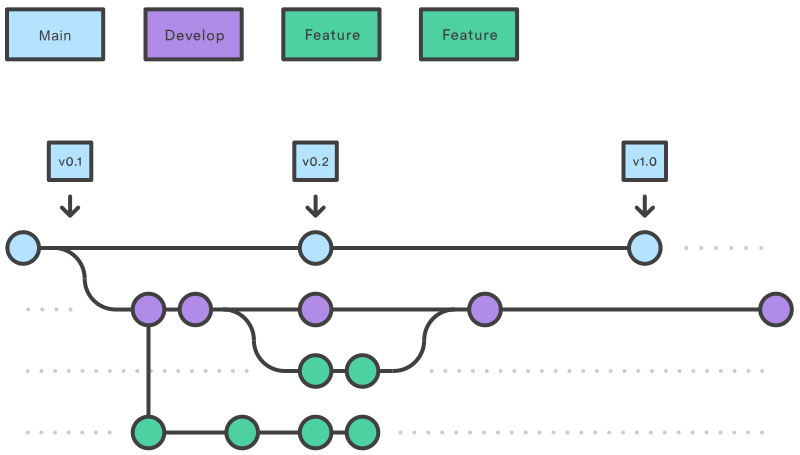
\includegraphics[width=\textwidth]{gitflow}
  \caption{Schematische Darstellung eines Git-Baums, der dem Standard von gitflow entspricht}
\end{figure}

Das Cloud-Team nahm eine Änderung am Schema vor und entfernte den branch develop, der angesichts der geringen Größe des Teams nicht relevant war.